\documentclass{article}
\usepackage{tikz}
\usetikzlibrary{mindmap}
\pagestyle{empty}
\begin{document}
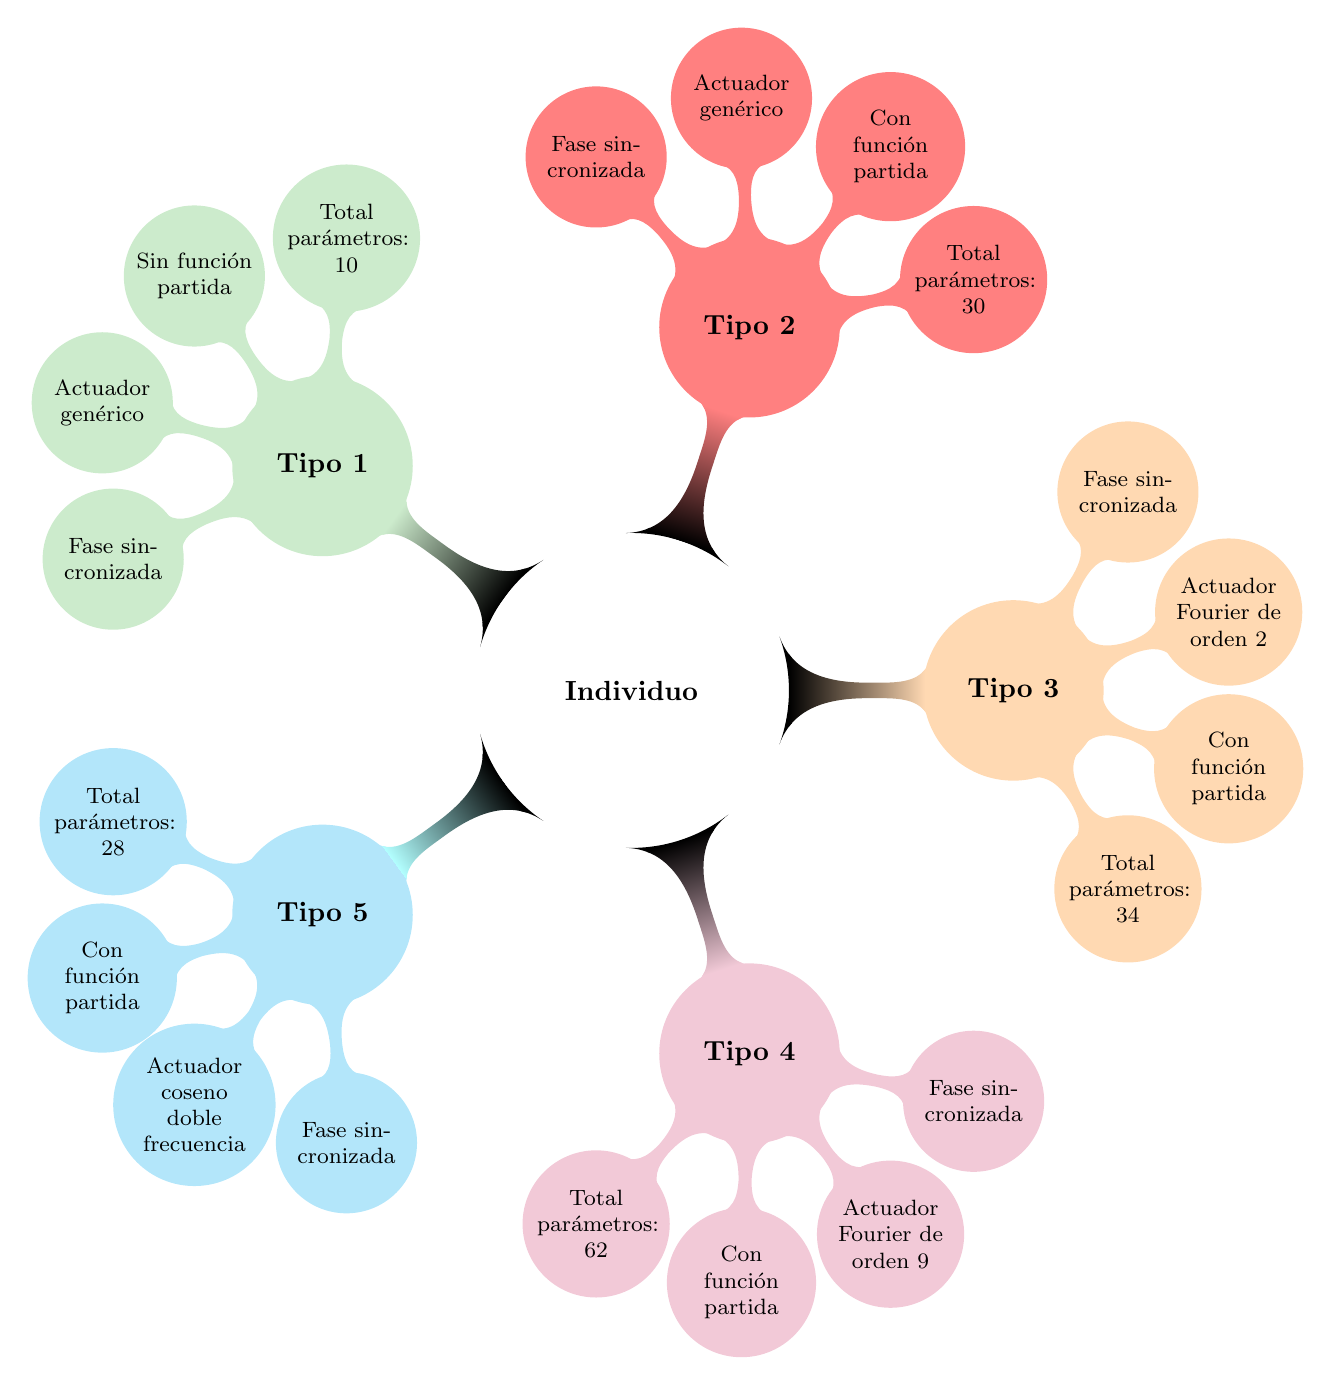
\begin{tikzpicture}[mindmap, grow cyclic, every node/.style=concept,  font=\bfseries,
    level 1/.append style={font=\bfseries,level distance=5cm,sibling angle=72},
    level 2/.append style={level distance=3cm,sibling angle=40},scale=0.97]


\node[color=white,text=black]{Individuo}
    child[concept color=cyan!30] { node {Tipo 5}
        child { node {Total par\'ametros: 28}}
        child { node {Con funci\'on partida}}
        child { node {Actuador coseno doble frecuencia}}
        child { node {Fase sincronizada}}
    }
    child[concept color=purple!70!white!30]  { node {Tipo 4}
        child { node {Total par\'ametros: 62}}
        child { node {Con funci\'on partida}}
        child { node {Actuador Fourier de orden 9}}
        child { node {Fase sincronizada}}
    }
    child[concept color=orange!30] { node {Tipo 3}
        child { node {Total par\'ametros: 34}}
        child { node {Con funci\'on partida}}
        child { node {Actuador Fourier de orden 2}}
        child { node {Fase sincronizada}}
    }
    child[concept color=red!50]  { node {Tipo 2}
        child { node {Total par\'ametros: 30}}
        child { node {Con funci\'on partida}}
        child { node {Actuador gen\'erico}}
        child { node {Fase sincronizada}}
    }
    child[concept color=green!60!black!20] { node {Tipo 1}
        child { node {Total par\'ametros: 10}}
        child { node {Sin funci\'on partida}}
        child { node {Actuador gen\'erico}}
        child { node {Fase sincronizada}}
    }
    ;    
    
\end{tikzpicture}
\end{document}